% Chapter Template

\chapter{Ensayos y resultados} % Main chapter title

\label{Chapter4} % Change X to a consecutive number; for referencing this chapter elsewhere, use \ref{ChapterX}

En este capítulo se detallan los resultados esperados y obtenidos sobre cada etapa del trabajo. A su vez, se indican las herramientas y metodologías empleadas en cada caso. Finalmente se expone el caso de uso completo integrando todos los componentes que integran al sistema.

%----------------------------------------------------------------------------------------
%	SECTION 1
%----------------------------------------------------------------------------------------

\section{Descripción del banco de pruebas}
\label{sec:bancoPruebas}

Para poder evaluar la detección, el seguimiento y la re-identificación de personas, se somete al sistema a una validación visual a partir del análisis de los videos procesados por cada parte del sistema. El sistema se evalúa en las siguientes etapas:

\begin{itemize}
\item Modelos de detección y seguimientos de personas.
\item Extractor de características.
\item Manejo de oclusiones y re-identificación de personas.
\end{itemize}

En la sección \ref{sec:validDetectorSeguidor} se detallan los criterios de validación empleados para evaluar los videos generados que se pueden observar en la figura \ref{fig:bancoPruebas}.

\begin{figure}[ht]
	\centering
	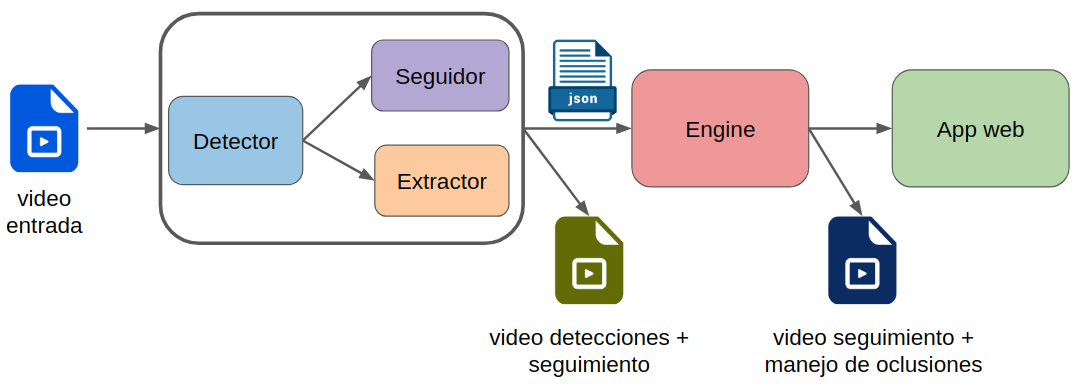
\includegraphics[scale=.50]{./Figures/bancoPruebas.png}
	\caption{Videos de ensayo generados en cada etapa.}
	\label{fig:bancoPruebas}
\end{figure}



Para poder evaluar la calidad del extractor de características, se creó un programa que facilita la captura de imágenes de personas en un video. En la figura \ref{fig:imagenesCrop} se pueden observar ejemplos de capturas realizadas de una misma persona en diferentes poses y locaciones a fin de generar un pequeño banco de imágenes de cada individuo. En la sección \ref{sec:validExtractor} se detallan los criterios de validación empleados para evaluar el extractor a partir del uso de estas imágenes.

\newpage

\begin{figure}[ht]
	\centering
	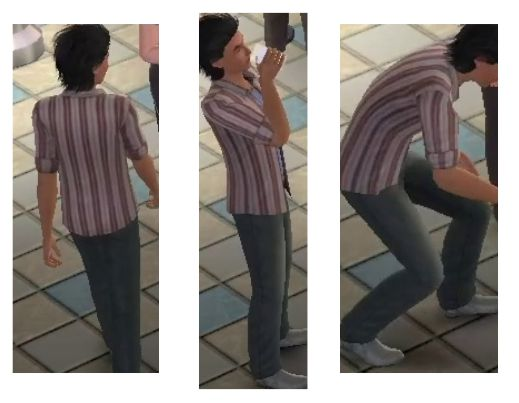
\includegraphics[scale=.45]{./Figures/imagenesCrop.jpg}
	\caption{Capturas tomadas de una persona.}
	\label{fig:imagenesCrop}
\end{figure}

De la experiencia obtenida de evaluar videos y el extractor de características, se desarrolló un programa capaz de automatizar los ensayos de validación del sistema. En la sección \ref{sec:precisionSistema} se detalla como se utilizó este programa para obtener métricas automáticas de la precisión de cada etapa y del sistema global.

%\newpage

%----------------------------------------------------------------------------------------
%	SECTION 2
%----------------------------------------------------------------------------------------

\section{Validación de los modelos de detección y seguimiento}
\label{sec:validDetectorSeguidor}

Validar sistemas de monitoreo por visión o procesamiento de imágenes normalmente implica una inspección manual por parte de un experto (conocedor del sistema y los objetivos a lograr) ya que es un proceso muy complejo de automatizar. El proceso empleado consiste en:

\begin{itemize}
\item Analizar si hay una zona de la cámara en donde las personas no están siendo detectadas.
\item Analizar si hay problemas de iluminación o de foco en los videos capturados.
\item Evaluar si las detecciones son continuas, o si las personas están constantemente cambiando de estado de detectada a no detectada.
\item Evaluar si hay falsos positivos, es decir, objetos que no son personas detectadas en el video.
\item Evaluar si el seguidor mantiene el mismo identificador para cada persona a medida que transitan por el recinto.
\item Detectar posibles oclusiones estáticas en el recinto que perjudiquen al sistema (por ejemplo un cartel que tape a las personas).
\item Evaluar con que frecuencia ocurre alguno de los desafíos conocidos en el seguimiento de cada persona (oclusiones, pérdidas o cambios de identificadores, personas que salen y vuelven a ingresar a cámara).
\end{itemize}

En la figura \ref{fig:fallasDetector} se pueden observar ejemplos de problemas que ocurren con el detector que precisan examinación manual.

%La figura \ref{fig:fallasDetector1de3}, \ref{fig:fallasDetector2de3} y \ref{fig:fallasDetector3de3}.

\newpage

\begin{figure}[!htpb]
     \centering
     \begin{subfigure}[b]{0.3\textwidth}
         \centering
         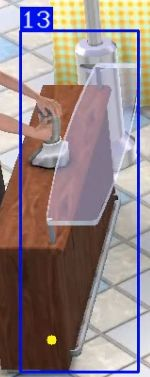
\includegraphics[width=.65\textwidth]{./Figures/fallasDetector1.jpg}
         \caption{Falsa detección.}
         \label{fig:fallasDetector1de3}
     \end{subfigure}
     \hfill
     \begin{subfigure}[b]{0.3\textwidth}
         \centering
         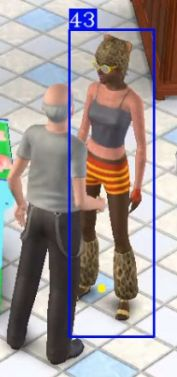
\includegraphics[width=.65\textwidth]{./Figures/fallasDetector2.jpg}
         \caption{No detección.}
         \label{fig:fallasDetector2de3}
     \end{subfigure}
     \hfill
     \begin{subfigure}[b]{0.3\textwidth}
         \centering
         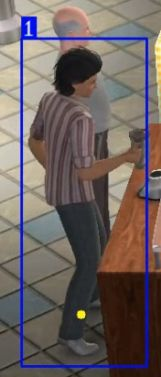
\includegraphics[width=.65\textwidth]{./Figures/fallasDetector3.jpg}
         \caption{Oclusión.}
         \label{fig:fallasDetector3de3}
     \end{subfigure}
        \caption{Fallas en la detección de personas.}
        \label{fig:fallasDetector}
\end{figure}

Es fundamental esta etapa de análisis porque permite entender las debilidades y fortalezas del sistema en una primera etapa de desarrollo.



%----------------------------------------------------------------------------------------
%	SECTION 3
%----------------------------------------------------------------------------------------

\section{Validación del modelo de extracción de características}
\label{sec:validExtractor}

Para evaluar la calidad del extractor de características no alcanzan las métricas de segmentación obtenidas en la sección \ref{sec:comparativaExtractores}. Es necesario llevar el concepto de re-identificación por vectores de características a algo tangible. Para ello, se creó un programa que permite realizar el seguimiento de personas únicamente por sus características, el cual se detalla en el diagrama de la figura \ref{fig:seguidorPorCaracteristicas}.

\begin{figure}[ht]
	\centering
	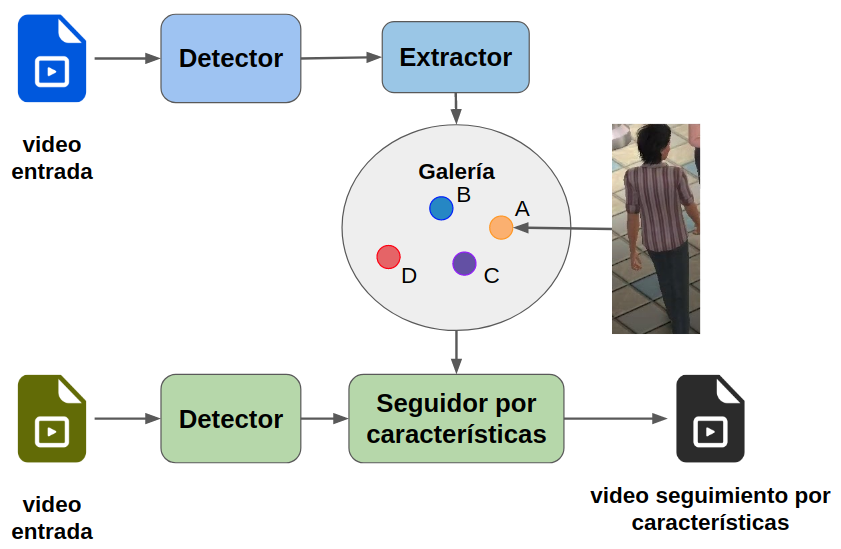
\includegraphics[scale=.60]{./Figures/seguidorPorCaracteristicas.png}
	\caption{Programa de seguimiento por características.}
	\label{fig:seguidorPorCaracteristicas}
\end{figure}

\newpage

El procedimiento llevado a cabo requiere dos iteraciones del video de entrada, en la primera se obtiene como salida la galería de características y en la segunda se obtiene el video de seguimiento por características.

Primera iteración del video:
\begin{itemize}
\item El sistema levanta las capturas de la imágenes de las personas y calcula los vectores de características de cada una.
\item Arma una galería de clusters de personas utilizando los vectores calculados.
\item Se analizan los clusters de la galería utilizando una herramienta que permite evaluarlos y graficarlos (ver figura \ref{fig:tsneClusers}).
\end{itemize}

\begin{figure}[ht]
	\centering
	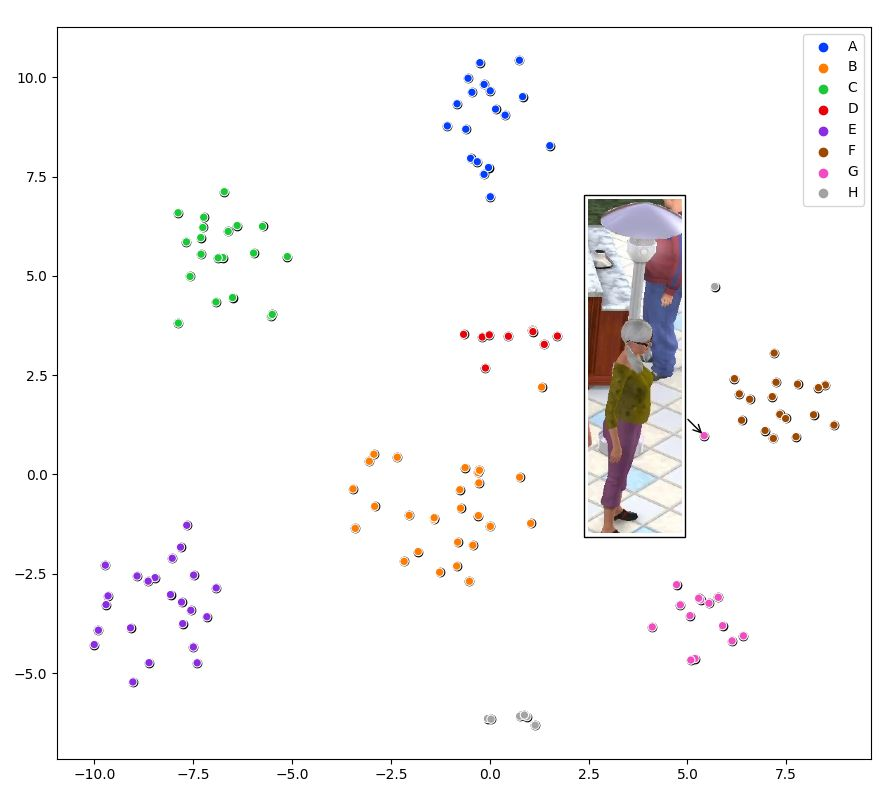
\includegraphics[scale=.60]{./Figures/tsneClusers.jpg}
	\caption{Análisis de los clusters generados.}
	\label{fig:tsneClusers}
\end{figure}

La herramienta para analizar clusters permite sacar conclusiones como las siguientes:
\begin{itemize}
\item No hay solapamiento de clusters en la galería y los clusters se encuentran bien separados.
\item Se puede observar que el cluster ``G'' tiene un vector muy cercano al cluster ``F'', debido a que dicho vector se calcula sobre una captura en donde ambas personas aparecen en la imagen.
\end{itemize}

\newpage

Segunda iteración del video:
\begin{itemize}
\item De cada detección reportada se extrae su vector de características.
\item El sistema toma cada vector de características y busca en la galería de clusters de personas a cual pertenece.
\item En caso de encontrar una persona candidata para esa detección, le asigna la letra de ese cluster.
\item Se genera un video de salida en donde las personas detectadas son representadas por las letras de los clusters candidatos.
\end{itemize}

La salida del sistema es un nuevo video con las detecciones de las personas. En vez de utilizar el seguidor para asignarles un identificador único a cada persona, se utiliza el procedimiento explicado en la figura \ref{fig:seguidorPorCaracteristicas} para asignar una letra a cada detección. En la figura \ref{fig:videoPorCaracteristicas} se observa un ejemplo del video resultante.

\begin{figure}[ht]
	\centering
	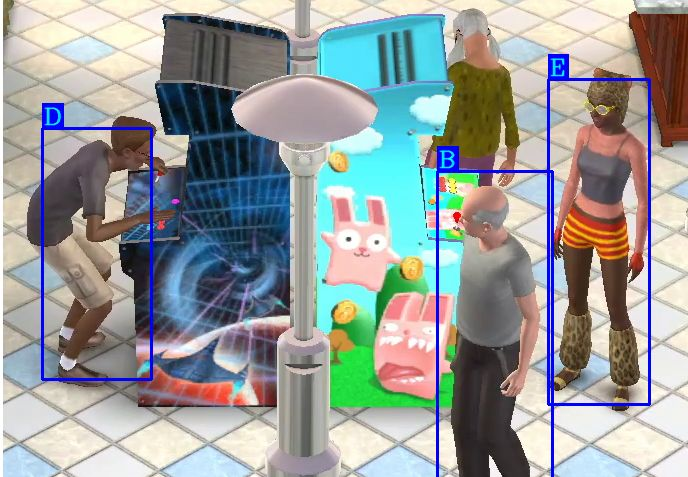
\includegraphics[scale=.60]{./Figures/videoPorCaracteristicas.jpg}
	\caption{Sistema de seguimiento por características.}
	\label{fig:videoPorCaracteristicas}
\end{figure}

Este proceso es muy robusto porque el sistema en la segunda iteración analiza el video conociendo de antemano las diferentes poses de cada persona, es decir, inicia el proceso con información futura. Las capturas de las personas se encuentran transformadas en clusters dentro de la galería. Por lo tanto, si la galería está correctamente armada se puede realizar seguimiento de personas por características sin errores. Utilizando este sistema se pueden obtener métricas automáticas de los videos obtenidos a la salida del Engine, por ejemplo:
\begin{itemize}
\item Cuánto tiempo fue monitoreada cada persona de forma correcta.
\item Cuántos identificadores distintos se asignaron a una misma persona.
\item Cuántos intercambios de identificadores hay en todo el video.
\end{itemize}

\newpage

%----------------------------------------------------------------------------------------
%	SECTION 4
%----------------------------------------------------------------------------------------

\section{Precisión de cada módulo del sistema}
\label{sec:precisionSistema}

Utilizando las métricas automáticas obtenidas en la sección \ref{sec:validExtractor} se puede validar por cada video procesado los siguientes requerimientos:
\begin{itemize}
\item Se considerará que una persona es correctamente monitoreada si al menos se mantuvo su seguimiento el 80\% del tiempo que circuló en el recinto.
\item Se considerará que el sistema funciona dentro de los parámetros aceptables si entre el 80\% y 100\% de las personas en el video fueron correctamente monitoreadas.
\end{itemize}

En la figura \ref{fig:metricasPorPersona} se observa el porcentaje de correcto seguimiento correspondiente a cada persona en el video luego de toda la cadena de procesamiento.

\begin{figure}[ht]
	\centering
	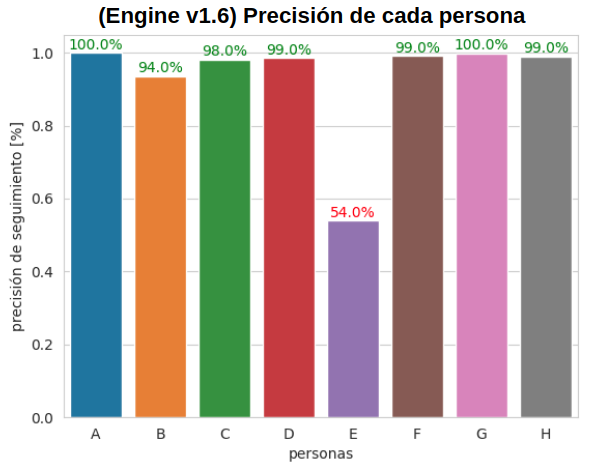
\includegraphics[scale=.80]{./Figures/metricasPorPersona.png}
	\caption{Precisión de seguimiento por persona.}
	\label{fig:metricasPorPersona}
\end{figure}

En la figura \ref{fig:metricasPorPersona} se observa que siete de ocho personas tienen una precisión de seguimiento por arriba del 80\%, y por lo tanto, la precisión total del sistema para ese video es de 87.5\%. 

En la figura \ref{fig:metricasPorSistema} se aplica la misma lógica para calcular la precisión de cada etapa del sistema y sus diferentes versiones para un mismo video de entrada.

\newpage

\begin{figure}[ht]
	\centering
	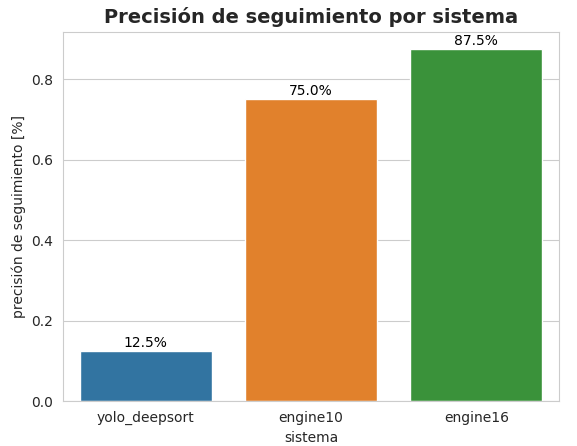
\includegraphics[scale=.80]{./Figures/metricasPorSistema.png}
	\caption{Precisión de seguimiento por sistema.}
	\label{fig:metricasPorSistema}
\end{figure}

Descripción de la evolución de los sistemas de la figura \ref{fig:metricasPorSistema}:
\begin{itemize}
\item Yolo y Deepsort: precisión que se alcanza si se utiliza el detector Yolo y el seguidor Deepsort tal cual se encuentra disponible en la web.
\item Engine10: precisión que se alcanza si al detector Yolo y al seguidor Deepsort se agrega el postprocesado del Engine v1.0 utilizando los vectores de características para el manejo de oclusiones y re-identificación de personas.
\item Engine16: precisión que se alcanza si al detector Yolo y al seguidor Deepsort se agrega el postprocesado del Engine v1.6 utilizando los vectores de características para el manejo de oclusiones y re-identificación de personas junto con la información agregada de las las zonas de interés.
\end{itemize}

En conclusión, la precisión del sistema aumenta con cada nueva funcionalidad que se incorpora. Por otro lado, en la figura \ref{fig:idSwitch} se observa que a medida que evolucionan los sistemas también se reducen los intercambios de identificador entre personas.

\newpage

\begin{figure}[ht]
	\centering
	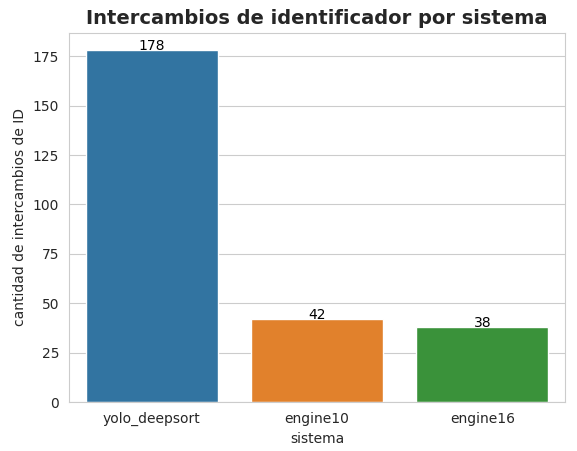
\includegraphics[scale=.80]{./Figures/idSwitch.png}
	\caption{Intercambios de identificador por sistema.}
	\label{fig:idSwitch}
\end{figure}

Con la última versión del Engine se logra alcanzar la precisión deseada de seguimiento, ya que con el agregado de las zonas se redujeron las falsas detecciones e intercambios de identificadores.

%----------------------------------------------------------------------------------------
%	SECTION 5
%----------------------------------------------------------------------------------------

\section{Simulaciones}
\label{sec:simulaciones}

Durante la realización de este trabajo no se tomaron muestras de videos de tiendas o recintos para realizar ensayos y validación, sino que se contó con el material de video disponible en internet. El problema es que la mayoría del material disponible es de muy corta duración (menor al minuto) o circulan muy pocas personas por el recinto (dos a tres personas). Debido a estos problemas fue muy difícil al comienzo validar las primeras etapas del trabajo.

El único video que se encontró en internet que cumpliera con todas las características fue un video de una tienda \citep{TIENDA_ORIGINAL} en donde aparecen más de 10 personas por más de un minuto. Este video se utilizó para las primeras demostraciones \citep{DEMO:1} con el fin de validar el sistema de re-identificación y manejo de oclusiones. El inconveniente con este video es que no resultó posible probar todas las funcionalidades de las zonas de interés. Principalmente, debido a que el espacio es bastante reducido y las personas durante la duración del video no llegan a transitar por más de una zona como se observa en la figura \ref{fig:tienda}.

\begin{figure}[ht]
	\centering
	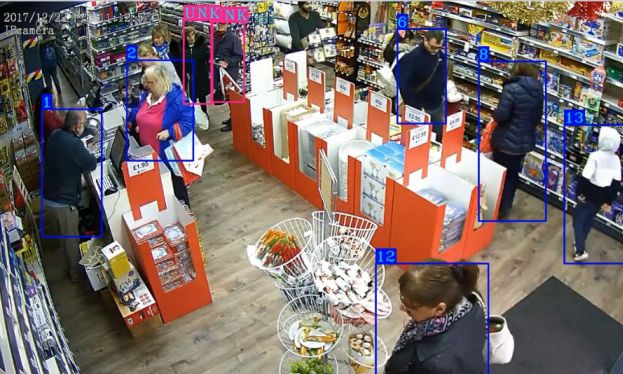
\includegraphics[scale=.70]{./Figures/tienda.jpg}
	\caption{Imagen del video de tienda utilizado al comienzo del trabajo.}
	\label{fig:tienda}
\end{figure}

\newpage

Dado que se necesitaba un video de un recinto con más zonas de interés y personas que se involucraran más con el espacio se buscó simular el entorno. Para ello, se optó por utilizar el videojuego "Los Sims 3" \citep{SIMS3}, en el cual es posible crear un ambiente totalmente a medida y personajes que interactúan en él. El juego permite crear personajes con diferentes personalidades por lo que cada uno interactúa de forma singular con el espacio pudiéndose obtener distintas métricas por el tiempo que se desee que dure el ensayo. En la figura \ref{fig:sims} se observa el entorno creado para ensayar las últimas funcionalidades creadas en el sistema, como por ejemplo las zonas de interés, las métricas y la aplicación web.

\begin{figure}[ht]
	\centering
	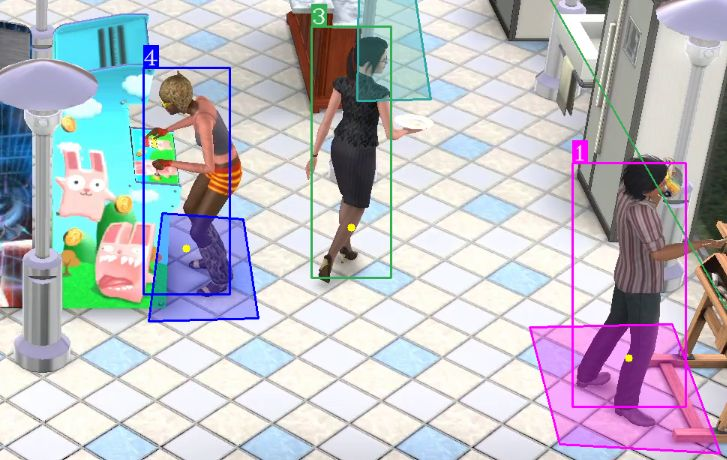
\includegraphics[scale=.50]{./Figures/sims.jpg}
	\caption{Imagen del escenario creado en el video juego "Los Sims 3".}
	\label{fig:sims}
\end{figure}

\newpage

El video generado a partir del simulador fue un éxito y permitió terminar de ensayar y validar todas las funcionalidades del sistema sin inconvenientes. En los primeros videos de simulación el detector apenas conseguía capturar a los personajes en el video, dado que la resolución de grabación y la calidad de las luces y sombras era baja. Se necesitó elaborar diez configuraciones diferentes de captura de video para que los colores y los personajes se vieran lo más realistas posible y el detector pudiera identificar a los personajes del juego como personas reales.

El resultado final \citep{DEMO:2} se acerca a un escenario real, ya que el detector presenta más inconvenientes detectando a los personajes que a las personas reales en la tienda y es por ello que la precisión de seguimiento utilizando solo el detector y seguidor para este video es muy baja. Finalmente, el video generado como una simulación pudo utilizarse luego de encontrar la configuración de video adecuada gracias a que el sistema de re-identificación ayuda a salvar todos los defectos del detector en el seguimiento de estos personajes ficticios.

%----------------------------------------------------------------------------------------
%	SECTION 5
%----------------------------------------------------------------------------------------

\section{Resultados}
\label{sec:resultados}

En esta sección se detallan los resultados y métricas obtenidas en la aplicación web luego de procesar el video de ``Los Sims'' con el Engine v1.6. En la aplicación web las detecciones y las personas se ejemplifican con figuras geométricas, ya que no se realiza la transmisión del video original en la misma; como se observa en la figura \ref{fig:simsWebApp}.

\begin{figure}[ht]
	\centering
	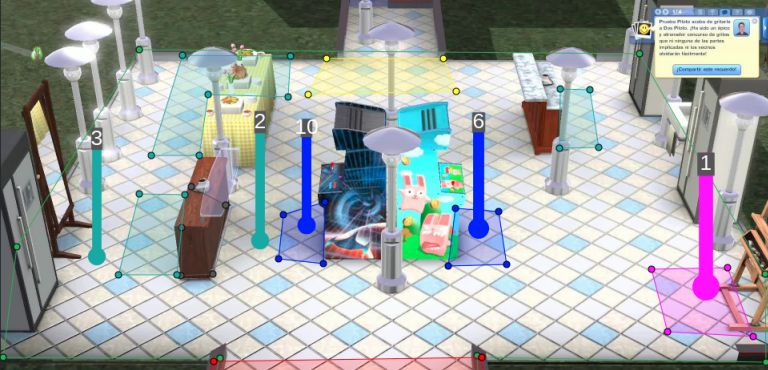
\includegraphics[scale=.60]{./Figures/simsWebApp.jpg}
	\caption{Imagen del monitoreo de personas en la aplicación web.}
	\label{fig:simsWebApp}
\end{figure}

Además de contar con el seguimiento y monitoreo de cada persona en la aplicación web, a la izquierda se cuenta con un panel que se actualiza en tiempo real en el cual se detallan las zonas con las cuales interactúo cada persona del recinto, como se observa en la figura \ref{fig:simsWebApp2}.

\begin{figure}[ht]
	\centering
	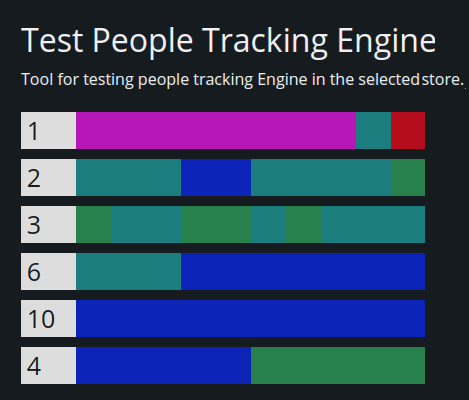
\includegraphics[scale=.80]{./Figures/simsWebApp2.png}
	\caption{Interacción de las personas con cada zona dibujada de interés.}
	\label{fig:simsWebApp2}
\end{figure}

\newpage

La aplicación web también arroja métricas sobre el recinto. Ofrece en una tabla cuales fueron las zonas más transitadas o más populares como también el mapa de calor del recinto (por donde caminaron las personas), como se puede observar en las figuras \ref{fig:metricasWebApp} y \ref{fig:metricasWebApp2} respectivamente.

\begin{figure}[ht]
	\centering
	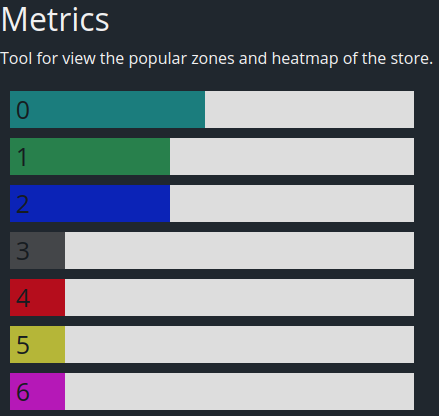
\includegraphics[scale=.80]{./Figures/metricasWebApp.png}
	\caption{Métricas de las zonas de interés del recinto.}
	\label{fig:metricasWebApp}
\end{figure}

\begin{figure}[ht]
	\centering
	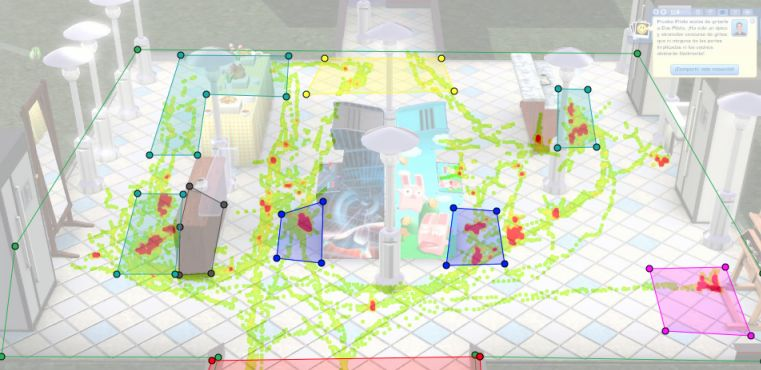
\includegraphics[scale=.70]{./Figures/metricasWebApp2.jpg}
	\caption{Mapa de calor del recinto.}
	\label{fig:metricasWebApp2}
\end{figure}

\newpage

De los resultados obtenidos se puede llegar a la conclusión que las zonas más visitadas del recinto son las zonas de comida y bebida (color cyan) y las zonas de juegos (color azul).